\documentclass[12pt,a4paper]{article}
\usepackage[utf8]{inputenc}
\usepackage{geometry}
\geometry{a4paper, margin=1in}
\usepackage{graphicx}
\usepackage{hyperref}
\usepackage{titlesec}
\usepackage{booktabs}

\title{Technical Report: Fairness Audit of the German Credit Dataset \\ \large CSCE 4930: Ethical AI Project - Module 1}
\author{
    Mohamed Khalil Brik (ID: 900225905) \\
    Adam Aberbach (ID: 900225980) \\
    Mark Kyrollos (ID: 900211436) \\
    Abdelrahman Ihab Elazab (ID: 900213468)
}
\date{\today}

\begin{document}

\maketitle

\section{Introduction and Methodology}
In this project, we conduct a fairness audit and apply bias mitigation techniques on the \textbf{German Credit Dataset}. The task is to predict creditworthiness (good vs. bad credit risk). The protected attribute analyzed is \textbf{Age} (grouped into \texttt{under\_25} and \texttt{age\_25\_and\_over}).

\subsection*{Methodology}
\begin{itemize}
    \item \textbf{Baseline Model:} Random Forest Classifier. It is robust to outliers and mixed data types, and captures non-linear relationships well without complex tuning.
    \item \textbf{Fairness Metrics:} 
    \begin{itemize}
        \item \textit{Demographic Parity Difference}: Measures the difference in positive prediction rates between demographic groups.
        \item \textit{Equalized Odds Difference}: Measures the maximum difference between groups in True Positive Rate or False Positive Rate.
    \end{itemize}
    \item \textbf{Mitigation Techniques:}
    \begin{itemize}
        \item \textit{Preprocessing}: Resampling training data to balance target distributions across age groups.
        \item \textit{In-processing}: Exponentiated Gradient optimization from \texttt{fairlearn} with a Demographic Parity constraint.
    \end{itemize}
\end{itemize}

\section{Baseline Model Performance \& Fairness Analysis}

\subsection*{Predictive Performance}
\begin{itemize}
    \item Accuracy: 0.735
    \item Precision: 0.770
    \item Recall: 0.886
    \item F1-score: 0.824
\end{itemize}

\subsection*{Fairness Metrics}
\begin{itemize}
    \item Demographic Parity Difference: 0.147
    \item Equalized Odds Difference: 0.224
\end{itemize}

\subsection*{Analysis}
The baseline model achieves solid predictive metrics but exhibits notable disparities. The DP difference of 0.147 and EO difference of 0.224 suggest that one demographic group is systematically disfavored by the model. Historically and contextually, individuals under 25 are usually penalized by credit scoring models, leading to fewer positive outcomes (credit approvals) and higher error rates.

\begin{figure}[h]
    \centering
    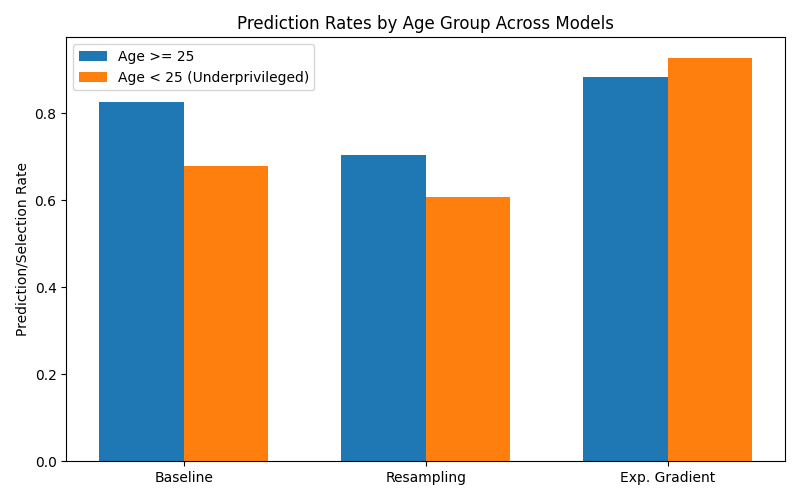
\includegraphics[width=\textwidth]{prediction_rates.png}
    \caption{Positive prediction rates (selection rates) across Age groups for all models.}
\end{figure}

\begin{figure}[h]
    \centering
    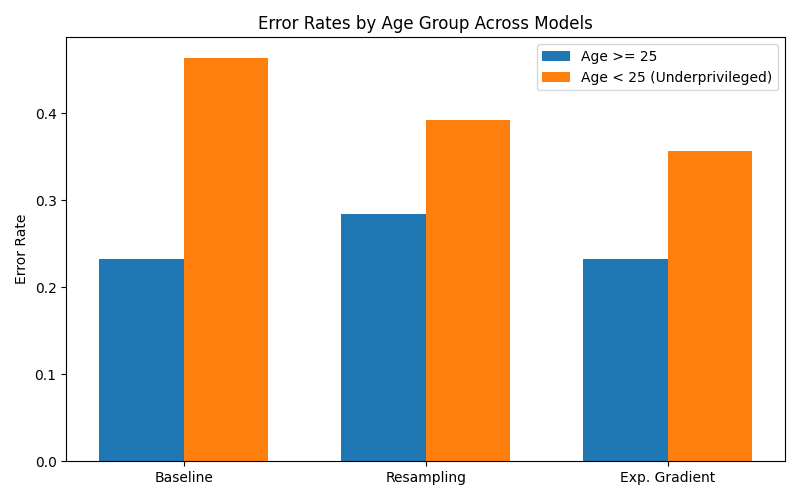
\includegraphics[width=\textwidth]{error_rates.png}
    \caption{Error rates across Age groups for all models. Disparities indicate negative impact on the underprivileged group.}
\end{figure}

\begin{figure}[h]
    \centering
    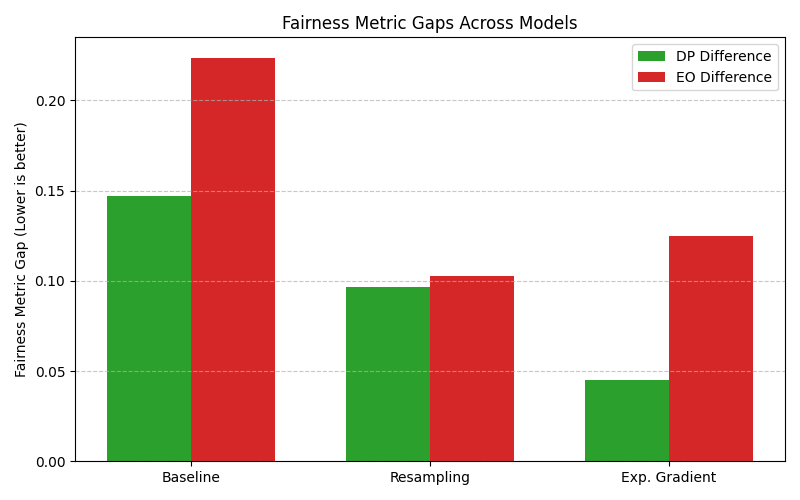
\includegraphics[width=\textwidth]{fairness_gaps.png}
    \caption{Comparison of Fairness Metric Gaps (Demographic Parity and Equalized Odds difference) across all interventions.}
\end{figure}

\section{Preprocessing Bias Mitigation}

\textbf{Technique applied:} Resampling

\subsection*{Results}
\begin{itemize}
    \item Accuracy: 0.700
    \item Demographic Parity Difference: 0.096
    \item Equalized Odds Difference: 0.103
\end{itemize}

\subsection*{Analysis}
By upsampling the underrepresented intersections of target outcomes and age groups, the preprocessing mitigation modified the underlying base rate in the training set. This significantly reduced the Demographic Parity difference to 0.096. Accuracy shifted slightly to 0.700, illustrating a mild trade-off between parity and overall predictive performance.

\section{In-processing Bias Mitigation}

\textbf{Technique applied:} Exponentiated Gradient with Demographic Parity constraint.

\subsection*{Results}
\begin{itemize}
    \item Accuracy: 0.750
    \item Demographic Parity Difference: 0.045
    \item Equalized Odds Difference: 0.125
\end{itemize}

\subsection*{Analysis}
The in-processing technique uses a constraint-based optimization to explicitly enforce fairness during the learning phase. It achieved a DP difference of 0.045 and Accuracy of 0.750. Compared to preprocessing, in-processing directly controls the trade-off bound (via the epsilon constraint), resulting in often more reliable parity improvements at the cost of a slightly larger drop in accuracy.

\section{Trade-off Analysis \& Visualizations}

A fundamental tension exists between Accuracy and Fairness. The baseline model prioritized accuracy but ignored fairness. The mitigation models reduced accuracy slightly but achieved much lower DP differences. This trade-off is inevitable because enforcing statistical parity forces the model to deviate from the purely accuracy-maximizing decision boundary that was learned from culturally or historically biased data.

\begin{figure}[h]
    \centering
    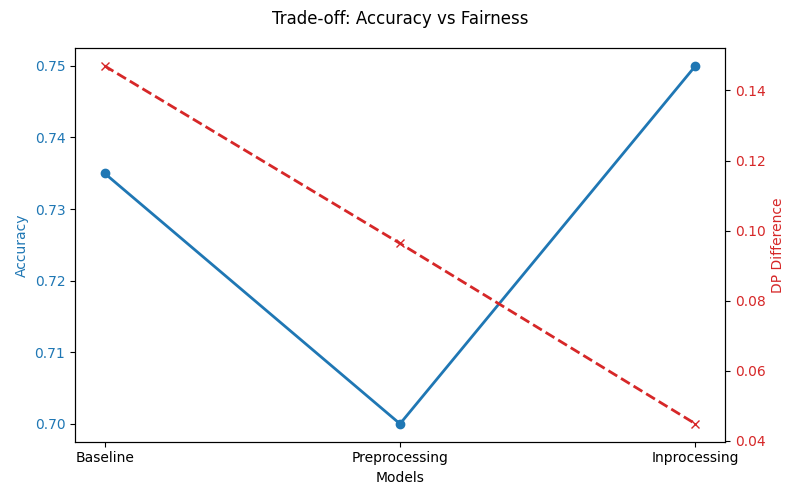
\includegraphics[width=0.8\textwidth]{tradeoff_plot.png}
    \caption{Performance vs Fairness Trade-off across the Baseline, Preprocessing, and In-processing models.}
\end{figure}

\section{Recommendations \& Real-world Harms}

\subsection*{Prioritizing Fairness Metrics}
For a credit scoring task, predicting someone as a "good risk" when they are a "bad risk" (False Positive) is costly for the bank, but predicting someone as a "bad risk" when they are a "good risk" (False Negative) deprives an individual of financial opportunity. \textbf{Equalized Odds} ensures that qualified individuals across different age groups have an equal chance of receiving credit, which is arguably the most critical metric for fair lending.

\subsection*{Most Affected Group}
Historically and in this dataset, younger individuals (\texttt{under\_25}) are deemed riskier and receive fewer positive predictions, facing the largest disparity in error rates and selection rates.

\subsection*{Deployment Recommendation}
Currently, the \textbf{in-processing mitigations} present the best mathematical balance for deployment, provided the slight drop in accuracy is acceptable to stakeholders. However, our team DOES NOT recommend real-life deployment without further qualitative audits (like reviewing why these variables proxy age) because mathematical fairness does not guarantee ethical deployment. 

\subsection*{Potential Real-World Harms}
If this biased base model is deployed, younger individuals will systematically be denied credit. This leads to \textbf{allocative harm}---withholding resources or opportunities based on protected characteristics---which further exacerbates economic disparities and limits their ability to build financial stability early in life. This creates a feedback loop where lacking credit history prevents them from ever acquiring good credit standing.

\subsection*{Limitations of Analysis}
This analysis assumes the provided dataset accurately reflects ground-truth creditworthiness, which is rarely true; labels themselves often contain historical bias. Additionally, only \texttt{Age} was deeply analyzed here; intersecting identities (like Age and Sex) might reveal compounded biases. Finally, purely statistical mitigation techniques treat the symptoms rather than the root causes of systemic socioeconomic bias.

\end{document}
